\documentclass[12pt,a4paper]{article} % Could set draft on here for more speed but no images
\usepackage[utf8]{inputenc}
\usepackage[english]{babel}
\usepackage{amsmath}
\usepackage{enumitem}
\usepackage{todo}
\usepackage{hyperref}
\hypersetup{
    colorlinks=true,
    linkcolor=blue,
    filecolor=magenta,      
    urlcolor=cyan,
}
\usepackage{amsfonts}
\usepackage{amssymb}
\usepackage{graphicx}
\usepackage[left=2cm,right=2cm,top=2cm,bottom=2cm]{geometry}
\author{Eric van der Toorn}
\title{Summaries}
\begin{document}
\maketitle
\section{Introduction}
I'll start with an introduction of my general ambition with this document, which is quite simply to record a personal summary and reflection for each of the books I've read or listened to. I have some catching up to do, and I'll start with outlining A. Why I'm doing this, and B. Which books I still have to do this for. Then I'll start with at least 2 of the books within this same paper before creating a structure, because I know from myself that I can get quite distracted/ dwell away from the main point if I do that first.
\subsection{Reasons}
This has been a thought in the back of my mind for a while, and it actually came up quite recently when I was having a discussion with Timotheos, a guest lecturer for the Growth: Managing Your Firm course. We were talking about some of the books we had read and I mentioned how it could get quite mixed up. Then he started talking about how he had a document which collected the books he had read (or at least a subset of them) with summaries and reflections. I agreed that it would be quite a useful thing, and he expounded with another reason: even if you stop with it, a few years later you may reread one of the books and close it with a different viewpoint, which you can then further reflect on. He also mentioned that the document he uses is not intended for modification, only being open for extension.
In general, I can tell for myself that the books I've read that I find useful get clearer in my memory when I focus on my specific memories of reading them, and that I actually feel excited for doing this kind of summary, so hopefully we'll have some fun doing this. I find that the more I write the more I am excited to write more, so let's continue!

\section{List of books}
It is hard to decide which books to do first, but I actually think I will treat it as a stack $->$ Last In First Out, as that way I can discuss the things that are most recent to me and best in my memory first. 
First a list of books that I am currently reading or want to read because they keep popping up in my head:
\subsection{Reading list}
\begin{itemize}
\item 12 Rules for Life (Jordan B. Peterson) - Quite the interesting guy talking about rules you can and should apply to your life
\item Predictable Irrational (Dr. Dan Aley) - Outlining some very interesting things in which humans are ever so irrational.

\item The Great Ideas of Psychology (Daniel N. Robinsson) [ON HOLD] - A summary of psychology from its very roots to its current state.
\end{itemize}
\subsection{Wish list}
\begin{itemize}

\item Black Swan, the impact of the highly improbable (...) [UNSTARTED] - ...
\item Zero to One - Dad really recommends this one
\item 50 lessons I learned from the world (Vic Johnson) - Interesting title and dad finished it
\item De meeste mensen deugen - Dad basically really admires the book
\item Homo Deus - All the other books of Harari have been great
\item Awaken the Giant within | Giant Steps (Tony Robbins) - Want to read and do this one during a vactation or when I have a span of free time large enough.
\item Nudge - Seems like a good book, was quite recommended
\item Find out anything from anyone ...

\end{itemize}
\subsubsection{Considering}
A list of books I'm considering, starting with the books recommended by Nadav (from Growth - Managing Your Firm)
\begin{itemize}
\item At the mind’s limits (Jean Amery)
\item Man’s search for meaning (Viktor Frankl)
\item Fear of freedom (Erich Fromm)
\item In the realm of hungry ghosts (Gabor Mate)
\item The abolition of man (CS Lewis)
\item I and Thou (Martin Buber)
\item Sovereignty of goodness (Iris Murdoch)
\item The malaise of modernity (Charles Taylor)
\item Intimate history of humanity (Theodor Zeldin)
\end{itemize}

\subsection{Read books}

\begin{itemize}
\item Mindset: The new Psychology of success. By Carol S. Dweck, a book expounding the Fixed and Growth mindsets.

\item Crucial Conversations, tools for talking when the stakes are high (Kerry Patterson, Joseph Grenny, Ron McMillan, and Al Switzler), a review on how the authors discovered that one of the major factors that makes people succeed in getting things done, both in business and elsewhere, was the ability to have crucial conversations.
\item Cognitive Behavioral Therapy (Dr. Sattersfield) -  A course on CBT, but still good enough that I feel like it requires a summary in order to remind myself of its major points
\item The 7 Habits of HIghly Effective People (Stephen R. Covey) - A book in which the author names and explains seven habits that are useful to apply, resulting in becoming more effective as a person. Interesting side note: first three are about the self, last four about interacting with others. You have to mold yourself before increasing your effectiveness(?) with others.
\item How to Talk to Anyone (Leil Lowndes) - 92 tips and tricks to interacting with others, some of which can actually be quite useful and fun to apply ;) Side note: will probably list all the tips shortly
\item The Wellbeing Quotient - Elements that contribute to my wellbeing
\item Leadership in a Complex World - A course I followed at the TU Delft as part of the honours programme; really fun and engaging, so I want to document what I learned here.
\item What the most successful people fo before breakfast (Laura Vanderkam) - Taught me the importance of a good morning ritual
\item No excuses  (Brian Tracy) - Quite a simple book on how you shouldn't blame things, just take responsibility or let it go (?)
\item The go-giver - how giving can be way more helpful than just taking - When done the right way
\item 21 lessons of the 21st Century (Harari) - About the general state of the present and the problems we're facing.
\item Homo Sapiens (Harari) - The past of humanity, beautifully given a new perspective
\item The Longevity Code (Kris Verburgh) - Basically my first non-fiction good book that I read for my pleasure and changed my life
\item Atomic Habits (James Clear) - This is slowly but surely changing my life for the better, learning how to approach changing habits.
\item The Subtle Art of not giving a fuck (Mark Manson) - Choose what you care about, don't let your environment choose for you.
\item Becoming (Michelle Obama) - First autobiography I've read afaik, and it was a great experience, think I'm a fan of hers now.
\end{itemize}

\subsection{Books that are complete and summarized}
Awfully empty to start with
\begin{itemize}
\item \ref{mindsets} Mindsets (Carol S. Dweck)
\item Talking To Strangers, (Malcolm Gladwell), a discussion on why we are so bad at perceiving people we don't know much about.
\item Thinking, Fast and Slow (Daniel Kahlemann) - Separates the mind into two parts, a fast intuitive mind and a slow rational one, and shows some very interesting aspects on the difference.
\end{itemize}


\section{Summaries}

\subsection{Mindsets (Carol S. Dweck) \label{mindsets}}

\textit{Maybe a bit cheating but I'll first copy my summary from last week here:}

In the book Mindsets, we learn about the two different mindsets people can have in a field: a fixed mindset where nothing can change and one must prove time and time again that the 'natural ability' was high enough, and the growth mindset, where everything is capable of growth if one tries hard enough in the right way.
A fixed mindset that can no longer breeze past an obstacle will fall, and fall hard, with no way to get back up.
Lacking talent cannot be overcome, and ways to avoid looking like you failed are created, for instance by not putting any effort in.
A growth mindset can also fall, but unlike the former they can always get back up again, knowing that trying harder or differently in order to grow the skills necessary in order to be able to overcome this obstacle in your way and continue on.
This allows the grower to maintain motivation and reach levels that the fixed-mind-setter is only able to dream of.


\subsection{Talking to Strangers (Malcolm Gladwell)}

I did not expect the content I got when I read this book. I expected it to be about some common fallacies we possess and tips on how to deal with them, but instead got a rollercoaster ride emotionally about how some fundamentally human flaws about understanding others contribute to a lot of despairingly solvable problems in our society. 
If I were to give the most powerful one to realise that would be the power of coupling, how certain actions are linked quite tightly with their environment and context. The example that Gladwell mentions is one that will stay with me for a very long time: The suicide of middle-aged women in England dropped significantly after one of the facourite methods for it was replaced (the town-gas that had carbon-monoxide inside and would lead to a 'clean' death by asphyxiation was replaced by modern gas which does not). Or how 90\% of the crime in a city usually centers around 5\% of the streets. Very eery to realise how we can make real life changing decisions like suicide or crime, because of a particular context. 

Gladwell wants us to realise that we are paradoxical in how we handle Strangers; for we understand/know that we ourselves are hard to read and understand but expect to exactly that for others.  To show this he took one of a lot of the psychological analyses that are quite vague and interpretable, like those 'What image do you see in this inksplash', and made some people do a 'complete the word' experiment where you would get a partial word and have to complete it, e.g. \_ \_ \_ v e $ \rightarrow $ k n i v e. When you ask people if you can draw conclusions about *themselves* they will well you that is no way to say anything about them, but if you ask them to do the exact same thing with someone else's results, they will happily draw the most extreme of conclusions. (this also ties into 'what you see is all there is' from Thinking, Fast and Slow)

When people perform counterintuitively to what our culture expects, they are quite quickly ousted or seen as 'strange', like the american student that got convicted (falsely) for murder because she had a different way of coping then she was supposed to have. 

One more interesting aspect that the book also touched upon is one that I believe is quite known to many in some ways: Alcohol transforms people, it doesn't reveal people. It was quite impressive to see that it actually made you adhere *more* to your environmental expectations instead of rebelling which is more in line with what I would have intuitively expected.

In conclusion, this book had a lot to tell, and tell it did. While some of the examples were more gruesome and criminal than others (we essentially went through a list of criminal cases), the way Gladwell extracts a message from these cases is quite compelling, though you should keep in mind that this book is mostly about awareness of our problems, not a set of solutions that we can always use. As always, the first step towards improving at something is to become aware of your current state and where the road forwards is. And in that I believe that Gladwell did quite well.

\subsection{Thinking, Fast and Slow (Daniel Kahnemann)}

This book tells us the story of three pairs of (opposing) entities: That of System 1 and System 2, Econs and humans, and the experiencing and remembering selves.
System 1 and 2 are personalisations of two kinds of ways our brain approaches the world, through an intuitive understanding of the world and speedy decisions (system 1), and a slower, (more) rational system 2, which monitors system 1 and may take over when it doesn't 'agree' or is triggered. Econs are completely rational beings who should be left free to make their own choices, Humans are not and should be given help when making some decisions (tldr; read nudge for this part)
The experiencing self is the human that experiences each moment while the remembering self remembers that and is usually more powerful in making decisions
It is a book about behavioural economics though I found it to be more fitting to decision psychology, as it pertains to how we make decisions and think about them.
The main theme of the book is how we're not rational (though Kahnemann wants to make sure we don't interpret that as meaning we're irrational).
Personally I found many of the examples in the book to be quite insightful and they stimulated me towards reflecting on my own perspectiv on the matters, so I'll take a few to highlight what I mean;


\begin{itemize}[leftmargin=4cm]
\item[Heuristics] When we get a question that is harder to answer and would require quite some thinking our intuitive system (system 1) will usually answer a simpler question and propose its solution instead. Think for instance if you are asked whether you are happy with your life it should take quite a while to collect all the factors which can influence that, but we can also just fill in whether we are happy right now.
\item[The law of small numbers] Extreme cases are more likely to occur when you're looking at small numbers
\item[Pain] Would it be more painful an experience to add onto a torture with the same peak pain an additional 10 minutes of a bit lesser pain? No, it would actually reduce the amount of pain someone remembers (remembering selves have no concept of time)
\item[Asian Disease problem] The way we frame two treatments will have influence on which solution will be chosen which has a paradoxical effect.
\item[Storylines] If you add 10 slightly worse years to someone's life they'll think the entire life's worse than without those years, because the end matters so much.

\end{itemize}


\subsubsection{Concepts named}
As this book is meant to be about learning the concepts and being able to use them, I would be remiss if I did not list them all out to increase the ability of myself to recall them :)

\begin{itemize}[leftmargin=4cm]
\item[Anchoring Effect] When we compare things any numbers that are given are used as a relative setpoint. e.g. If we see a house on sale for 2 millions we'll go lower from there not get an entire different start bid like 2 tons. 
\item[Sunk Cost] Basically the gambler's fallacy, we shouldn't consider what we have already spent when making a choice, just the current state of things.
\item[Loss Aversion] All things considered, losses weigh more than gains both in the amount of emotion they cause and the amount of regret they spark. As such we tend to avoid sure losses and take gambles, while the opposite is the case for gains.
\item[Regression to mean] Luck/chance has a larger role in life than we'd usually like to imagine, which ends up to mean that if something goes well occasionally, that it will also go bad occasionally.
\item[Framing bias] Framing a question one way or another can influence how it is perceived (as a positive or negative outcome, good or bad solution)
\item[Availability bias] When asked how frequently something occurs, you'll think it occurs more frequently if it comes to mind more easily (think terrorist attacks)
\item[Cognitive load] We tend towards less cognitive load (stress on the brain). If something takes a lot of brain power, we'll want to avoid it more.
\item[The Confirmation bias] We tend to look for info that reinforces our own beliefs instead of adapting your beliefs to other facts which we tend to overlook.
\item[Correlation != Causation] No more need be said here
\item[Substitution] Answer a harder question with an easier one (sometimes without knowing)
\item[Causes $>>$ Facts] Humans don't want statistics, they want a sappy story.
\item[Halo effect] Kinda seeing things as black and white. Your first impression colours the story you draw of someone.
\item[Environmental bias] Your surroundings effect you more than you'd want to admit. A lot of posters of the great leader will tend to make you more loyal, sad to say.
\item[Less is more] If you add more detail to a situation you make it seem more likely while you actually reduce the probability (subsets!)

\end{itemize}

\paragraph{More info?}
Could always re-read the book, and I found that the following medium article was quite clear: \href{https://medium.com/swlh/every-chapter-of-thinking-fast-and-slow-in-7-minutes-5e6adf89cf39}{Every Chapter of Thinking Fast, and Slow in 7 Minutes}
\begin{figure}
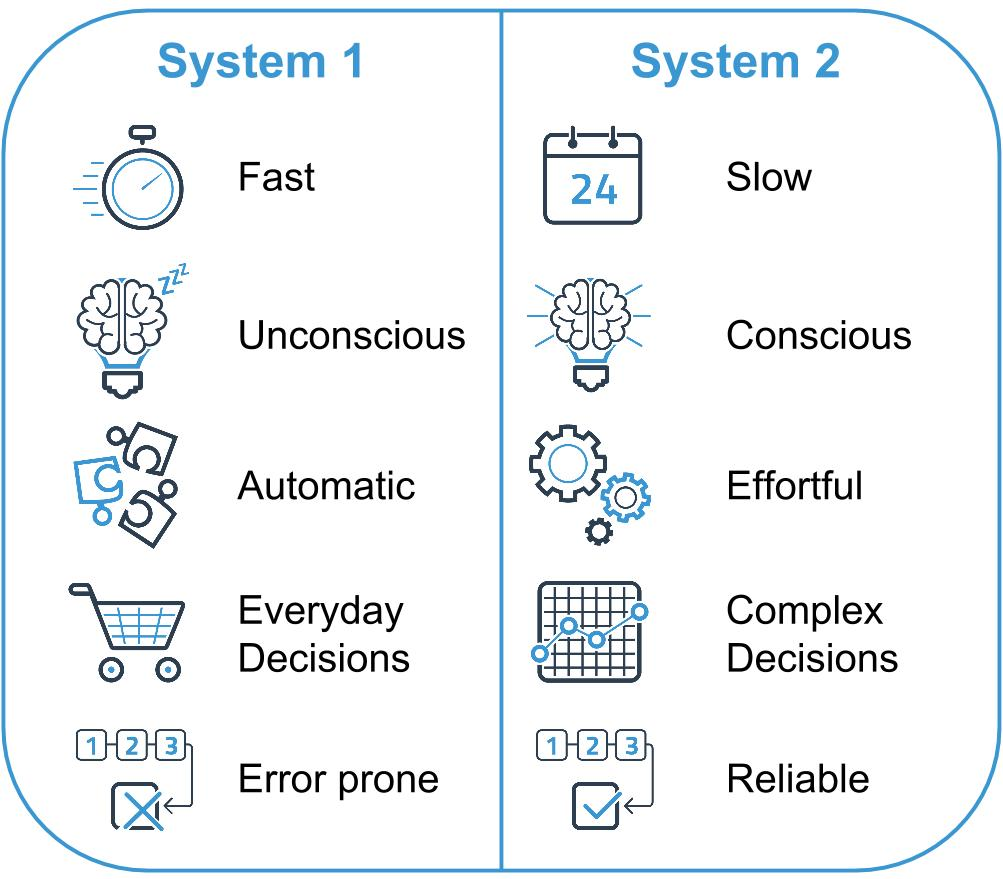
\includegraphics[scale=0.5]{summaries/thinking-fast-and-slow-systems.png}
\caption{The systems of the mind (useful overview)}
\end{figure}

\subsection{De meeste mensen deugen (Rutger Bregman)}

I'm going to be honest here, I never expected to be putting a Dutch book on this list. Not because I can't read Dutch 
(I have a good grasp of the intricacies of the Dutch language as a native), but because I had grown to hate Dutch literature in all of its forms over the years in high school where I was forced to read and analyze literature that I intensely disliked, which took away my interest. "Is this the best that Dutch literature can offer me," is the thought that recurred time and again. 
My prime example, by virtue of its still-living memory, is not a particularly horrific one but a work that started off great. 'Het Leven in een dag' is a novel that describes how life could look like if we were to live in a world that where lifespans where compressed to a single day, and everything was about 'firsts,' from the first time you saw the sun rise to the first time you had sex. Firsts were also lasts however, and most things could never happen again (we conveniently exclude things like breathing and thinking). In this world, heaven is a single moment where 'everything' happens, and hell is the endless repetition (or 'Earth' for those less religiously inclined) The concept is quite interesting and sets one to thinking about how the repetition of events makes them lose a lot of their magic. The plot of the story was that of a typical romance with an interesting plan: Have more sex by going to hell. In our world the reverse is usually preached, but I like this version more to be completely honest. The plan to go to hell by murdering someone and getting executed succeeds and our main character finds himself on Earth and looks around for his girl.

Then, to completely gore the entire thought process that the first two-thirds of the book stimulate one too, the main character is recruited by the man he killed to become, of all things, a prostitute. The following few scenes are just raunchy depictions of the things he is all but forced to participate in, my 'favourite' being where he has an orgy while skydiving, laid out in explicit detail. 

I realise that I have in the process of wanting to rant about it written an entire review, so I'll now start talking about the book that (after a lot of stimulation from my dad and it being suggested by a lady I met while traveling) I reluctantly started listening to and now am determined to finish to the end, though I sometimes have to bite through some reluctance. 

The book starts off discussing how humanity is perceived, from a philosophical perspective. The age-old question that Bregman wishes to touch upon once again (and hopefully answer) is whether civilization - rules, order, and leadership - is a boon to humanity, a requirement for proper treatment of others, or a poison that has only eroded the basic human decency that is inherent to all of us.

Bregman wants to approach this topic, which is prone to being quite subjective, as scientifically as possible. I believe he did a remarkable job, though the book \textbf{is} named after his opinion, which is that humans are inherently decent. He starts by analyzing our behaviour without civilization, through pre-historical findings, current tribes, and stories where civilization got a 'fresh start' - a la The Lord of the Flies - then continues onto social psychological conclusions that are widely known but deeply controversial, to finish with how things should change if the worldview that most people are decent would be implemented, and what would be the effect. In the conclusion he briefly describes 10 lessons he's learned over his research.

In his efforts to sound rational and scientific he has done quite well, though some parts of the book leave me wondering whether he sufficiently defuses the arguments against human cruelty being non-inherent. One thing that I feel he skirts about unwilling to actually dive into is the belief that civilization is responsible for all that is cruel. He repeatedly paints the civilized world as the 'evil' guy, with its colonization and slavery practices, through the comparisons feel more like comparing apples to oranges. I would've enjoyed it if he'd mentioned more cases where one civilization compared to another. Are leaders always the people with the most hate for eachother? How does this work in rebellions? How should we look at people that commit not violent crime but horrible deeds like paedophilia? These are just some of the questions that the book neglected to touch upon in what felt like an effort to not get into the intricate debates surrounding those topics. 

To conclude my review, this book has made a significant impact on how I perceive the world in terms of how people are, baring some of the resolutions that I felt are intuitive, and with that allowing me to become more resolved in their veracity. On the other hand, it is like an opening move at a debate, where the response and the ensuing persuasive efforts still have to follow. And I am looking forward to see the arguments from both sides.

\subsection{Loserthink (Scott Adams)}

Never thought I'd be reading a book that puts Trump in a mostly positive light and not feel like the author doesn't know anything.
Scott Adams made for a very interesting read about his concept of losethink. Loserthink being basically anything that doesn't help you, society, or your current conversation in any meaningful way.

\subsubsection{Summary of learning points}
Adams' approach was to go through the 'minds' of particular professions who each have particular methods for perceiving the world and seeing what we can learn from them.
\begin{itemize}
    \item Psychologist:
    \item Scientist
    \item Exonomist
    \item Historian
    \item Artist
    \item Leader: compare your plan to the next best one
\end{itemize}

Followed by a chapter of persuasion items that do not contribute (things done by political pundits that you shouldn't)


\subsection{Moonwalking with Einstein (todo author)}

\todo[inline]{Write this}

\subsection{Range: Why Generalists thrive in a Specialized World (David Epstein)}

This was one of those nice reads that makes everything it says stand out as well-founded.
The main point that the author tries to make is that you should not specialize (early),
as it can be just overvuew that you gain by keeping a broader perspective that allows you to succeed.
He illustrates this with several topics: Sports, Art, Music, Study (choice), and (academic) research.
The 'antagonist' is presented in the introduction: the 'kind' world of Tiger Woods, who succeeded because he specialized early.
Epstein argues that this is the exception rather than the rule, and there are many more stories of athletes with 'range': 
They initially explore a braoad range of sports and only after some time (quite late by some measures), fo they delve into one and invest.
Some other quick main points:
\begin{itemize}
\item Start broad, specialize late $\rightarrow$ T-shaped learning
\item Use analogical thinking (like Kepler)
\item Communication is key (an example of the shuttle crash from NASA is given), and don't become too quantative.
\item Plan for short-term not long term (example of a famous female CEO is given, who got where she is by constantly planning short-term)
\begin{itemize}
    \item I'm not too sure how to think of this, as it kinda also invalidates everything about following your dreams.
\end{itemize}
\item Do what you feel passion for now, no when to change. Doesn't mean giving up on having a bad day.
\item Creativity can be found in applying old things to new problems, or new things to old problems,
\item Learn to estimate (like someone from the Manhattan project)
\item We live in a wicked world, not a kind one (reference to Kahnemann)
\item We're getting better at abstract thinking, learn more about Reasoning and Logic.
\end{itemize}

One thought that I got left with is what this entire story implies for the role of guidance. 
If you must let everyone explore as much as they want, can you still guide your e.g. children in some way? 

\end{document}